% Definición
\documentclass[12pt]{beamer}

% Paquetes
\usepackage{graphicx,listings}
\usepackage[utf8]{inputenc}
\usepackage[spanish,es-tabla]{babel}
\usepackage{times}          % Usar tipo Times-Roman
\usepackage[T1]{fontenc}    % Usar la codificación T1

% Datos
\title{Metodología Running Lean aplicada a un lector de noticias inteligente}
\author{Andrés M. Jiménez Ríos}
\institute[TFM]{Trabajo Fin de Máster}

% Temas
\usetheme{Boadilla}
\usecolortheme{crane}
\useoutertheme{infolines}
\useinnertheme{rectangles}

% Paquetes
\usepackage{lmodern,textcomp}
\usepackage{smartdiagram}

% Opciones
\setbeamertemplate{navigation symbols}{}
\setbeamertemplate{button}{\tikz
     \node[
     inner xsep=10pt,
     draw=structure!80,
     fill=structure!50,
     rounded corners=4pt]  {\Large\insertbuttontext};}


\lstset{
	literate={á}{{\'o}}1
	{é}{{\'e}}1
	{í}{{\'i}}1
	{ó}{{\'o}}1
	{ú}{{\'u}}1
}


\AtBeginSection{ 
	\begin{frame}{Índice} 
		\tableofcontents[currentsection]
	\end{frame}
}

\AtEndDocument{
	\frame{\titlepage}
}

% Inicio
\begin{document}

% Diapositivas
	\frame{\titlepage}
	
	\begin{frame}{Índice}
		\tableofcontents
	\end{frame}

	\section{Introducción}	
		\begin{frame}{\textit{Running Lean}}
			\begin{block}{}
				\textit{Running Lean is a systematic process for iterating from Plan A to a plan that works, before running out of resources.}
			\end{block}
			\begin{block}{Influencia}
				\begin{itemize}
                    \item Steve Blank - \textit{Customer Development}
                    \item Eric Ries - \textit{Lean Startup}
                    \item Alex Osterwalder - \textit{Bussiness Model Canvas}
                \end{itemize}
			\end{block}
        \end{frame}
	
		\begin{frame}{Periodismo}
			\begin{block}{Situación actual}
				La falta de contenido de calidad, las redes sociales y las \textit{fake news}.
			\end{block}
			\begin{block}{Mundo digital}
				Su propuestas son la sindicación de contenido, las redes sociales y aplicaciones propias.
			\end{block}
		\end{frame}

		\begin{frame}{Propuesta}
			\begin{block}{}
				Estudio y aplicación de la metodología \textit{Running Lean}.
			\end{block}
			\begin{block}{}
				Análisis de los problemas actuales del periodismo digital.
			\end{block}
			\begin{block}{}
				Realización de una aplicación que implemente las propuestas.
			\end{block}
		\end{frame}

		\begin{frame}{Alternativas}
			\begin{columns}[onlytextwidth]
				\begin{column}{0.3\textwidth}
					
\includegraphics[width=\textwidth,height=0.8\textheight,keepaspectratio]{img/alternativas/feedly_logo}
				\end{column}
				\begin{column}{0.3\textwidth}
					
\includegraphics[width=\textwidth,height=0.8\textheight,keepaspectratio]{img/alternativas/flipboard_logo}
				\end{column}
				\begin{column}{0.3\textwidth}
					
\includegraphics[width=\textwidth,height=0.8\textheight,keepaspectratio]{img/alternativas/gnews_logo}
				\end{column}
			\end{columns}
		\end{frame}
	
	
	\section{Estudio}
		{
			\usebackgroundtemplate{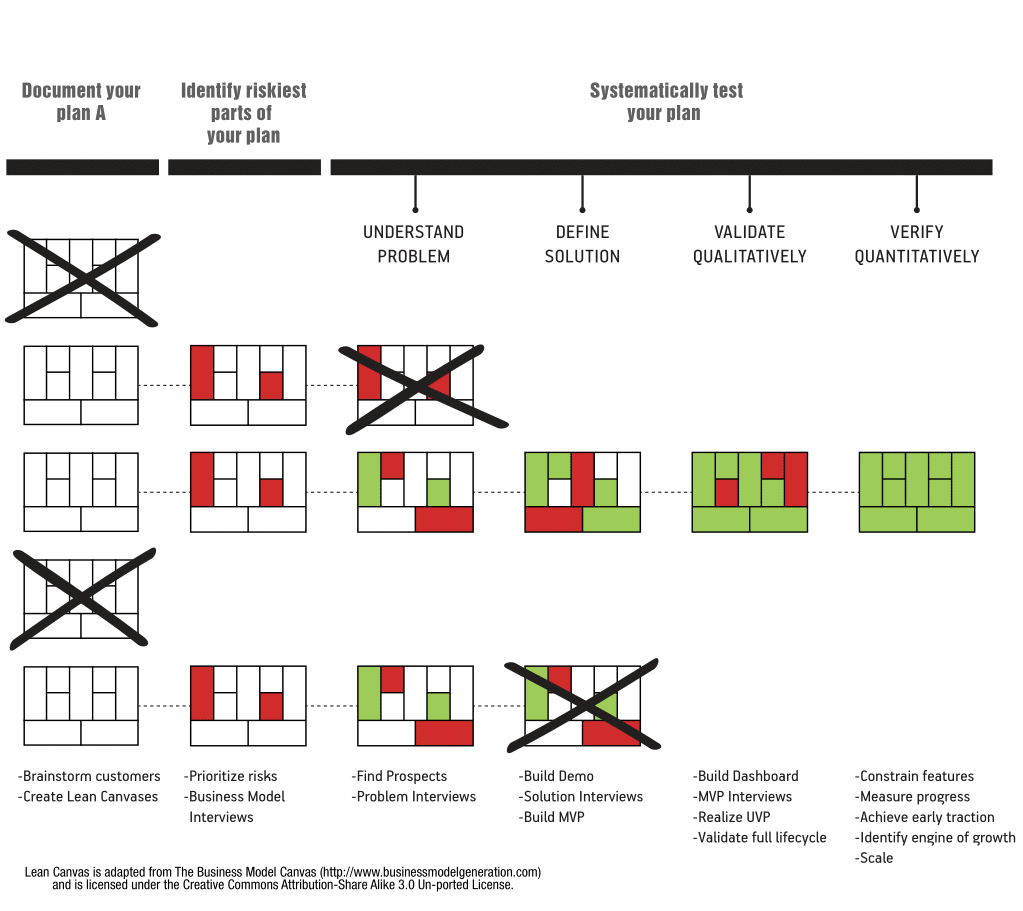
\includegraphics[height=\paperheight,width=\paperwidth]{img/lean/running_lean}}
			\setbeamertemplate{navigation symbols}{}
			\begin{frame}[plain]
			\end{frame}
		}

		\begin{frame}{Canvas inicial}
            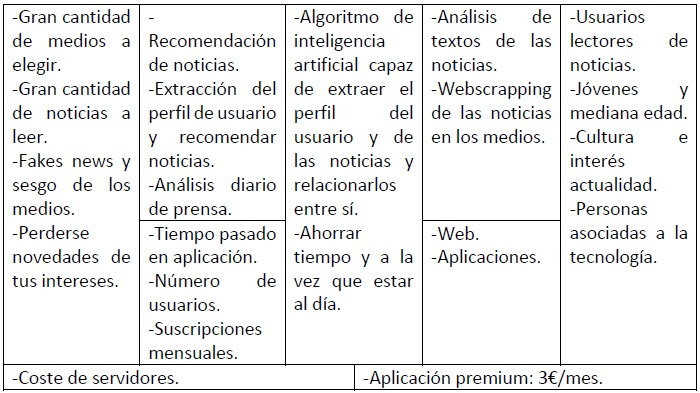
\includegraphics[width=\textwidth,height=0.8\textheight,keepaspectratio]{img/canvas/canvas_inicial}
        \end{frame}

		\begin{frame}{Hipótesis de problemas}
			\smartdiagramset{
				bubble center node font = \scriptsize,
				bubble node font = \scriptsize,
				bubble center node size =2.5cm,
				bubble node size =1.75cm,
			}
			\tikzset{bubble node/.append style={text width=1.75cm,align=center}}

			\begin{center}
			\smartdiagram[bubble diagram]{
				Preocupación del usuario, Gran cantidad de noticias, Objetividad de las noticias, Seguimiento de temas}
			\end{center}
        \end{frame}

        \begin{frame}{Iteraciones realizadas}
            \resizebox{\textwidth}{!}{
                \begin{tabular}{*5c}
                    \hline
                    \textbf{Iteración} & \textbf{Hipótesis} & \textbf{Fechas} & \textbf{Tests} & \textbf{Resultado} \\
                    Problema 1 & Primera hipótesis & S/29-09 & 2 entrevistas & No aplica \\ 
                    Problema 2 & Primera hipótesis & S/06-10 & 4 entrevistas & Se confirma \\ 
                    Problema 3 & Segunda hipótesis & S/13-10 & 4 entrevistas & Se confirma \\ 
                    Problema 4 & Tercera hipótesis & S/20-10 & 143 encuestas & No se confirma \\ 
                    Solución 1 & Soluciones & S/27-10 & 4 entrevistas & Se confirma \\ 
                    \hline
                \end{tabular}
            }
        \end{frame}
        
		\begin{frame}{Canvas final}
            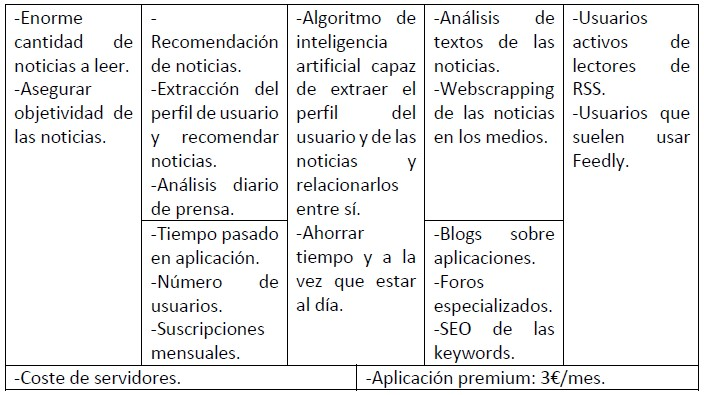
\includegraphics[width=\textwidth,height=0.8\textheight,keepaspectratio]{img/canvas/canvas_final}
		\end{frame}
	
	\section{Planificación}
		\begin{frame}{Metodologías}
			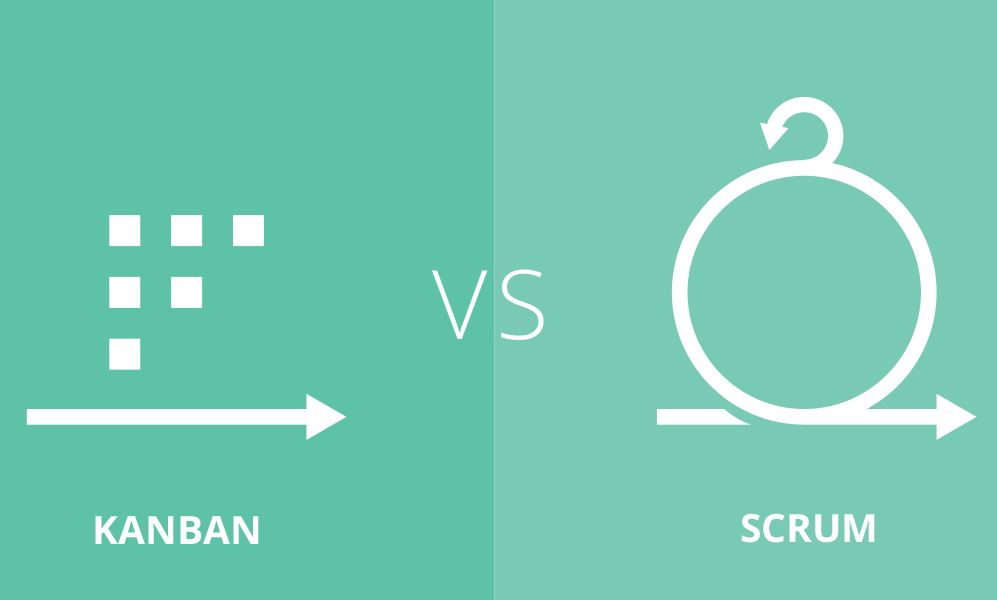
\includegraphics[width=\textwidth,height=0.8\textheight,keepaspectratio]{img/scrum/scrum_vs_kanban}
		\end{frame}

        \begin{frame}{Planificación Temporal}
            \resizebox{\textwidth}{!}{
                \begin{tabular}{llrrr}
                    \hline
					\textbf{ID} & \textbf{Nombre} & \textbf{Estimación} & \textbf{Duración} & \textbf{Variación} \\
					S0 & Fase previa & 70:00:00 & 66:57:53 & 4,34\% \\
					S1 & Investigación & 30:00:00 & 60:26:29 & -101,47\% \\
					S2 & Funcionalidad completa & 100:00:00 & 70:26:20 & 29,56\% \\
					S3 & Virtualización de los servicios & 30:00:00 & 46:58:15 & -56,57\% \\
					S4 & Capa Inteligencia Artificial & 70:00:00 & 55:57:54 & 20,05\% \\
					& & \textbf{300:00:00} & \textbf{300:46:55} & \textbf{-0,26\%} \\
                    \hline
                \end{tabular}
            }
        \end{frame}

        \begin{frame}{Planificación Económica}
            \resizebox{\textwidth}{!}{
                \begin{tabular}{lrr}
                    \hline
					& \textbf{Coste total} \\
					Personal & 3.755,47€ \\
					Hardware & 309,58€ \\
					Software & 471,61€ \\
					
					\hline
					Subtotal & 4.536,65€ \\
					Contingencias & 680,50€ \\
					\textbf{Total} & \textbf{5.217,15€} \\
                    \hline
                \end{tabular}
            }
        \end{frame}
	
	\section{Diseño}
		{
			\usebackgroundtemplate{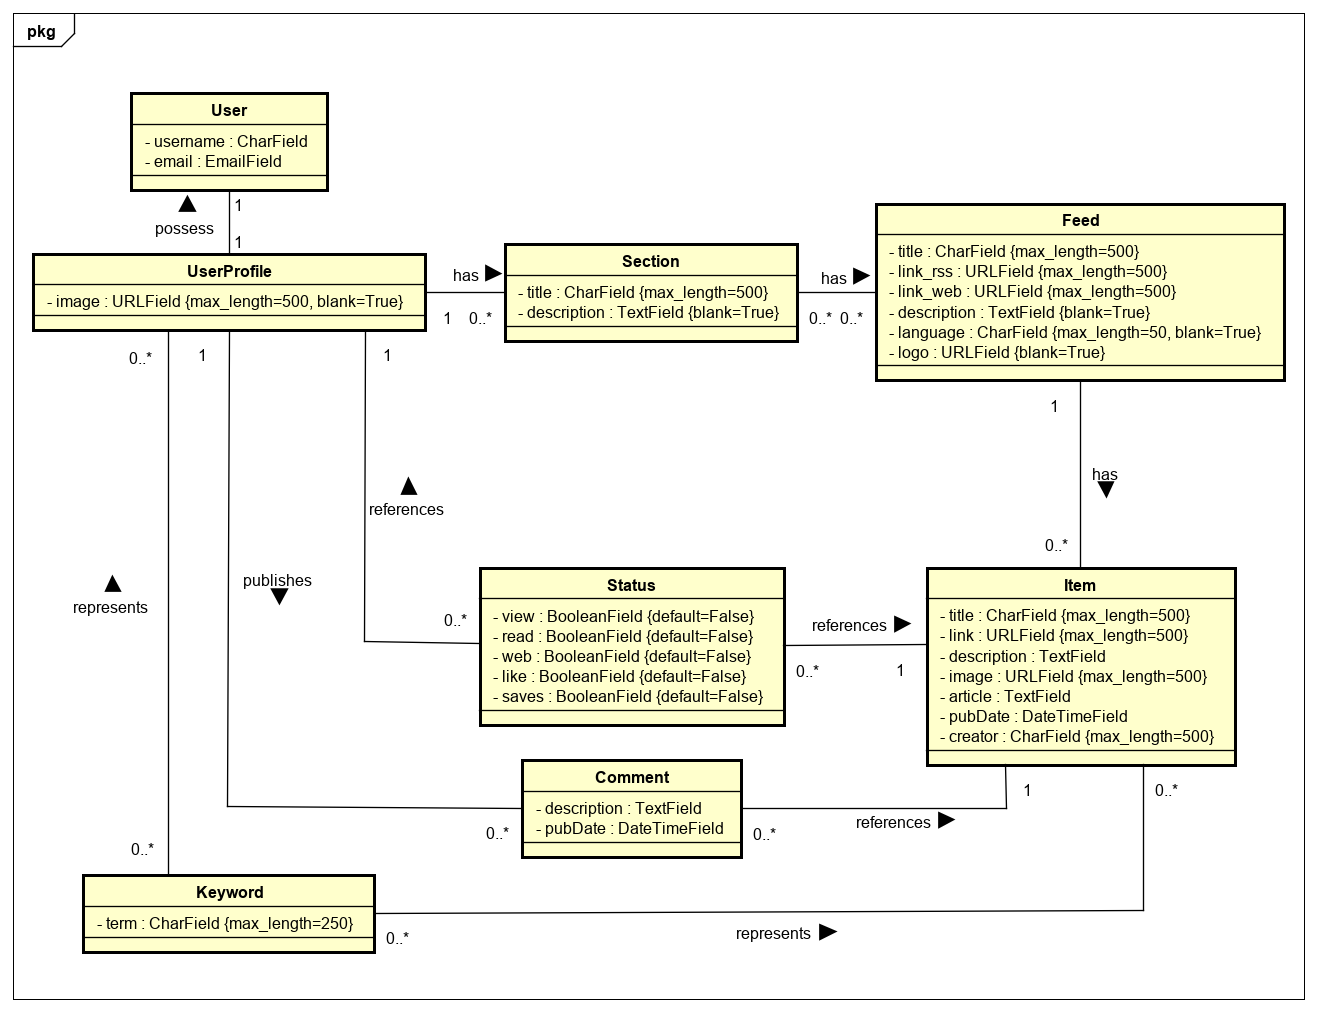
\includegraphics[height=\paperheight,width=\paperwidth]{img/diagram/class_diagram}}
			\setbeamertemplate{navigation symbols}{}
			\begin{frame}[plain]
			\end{frame}
		}

		{
			\usebackgroundtemplate{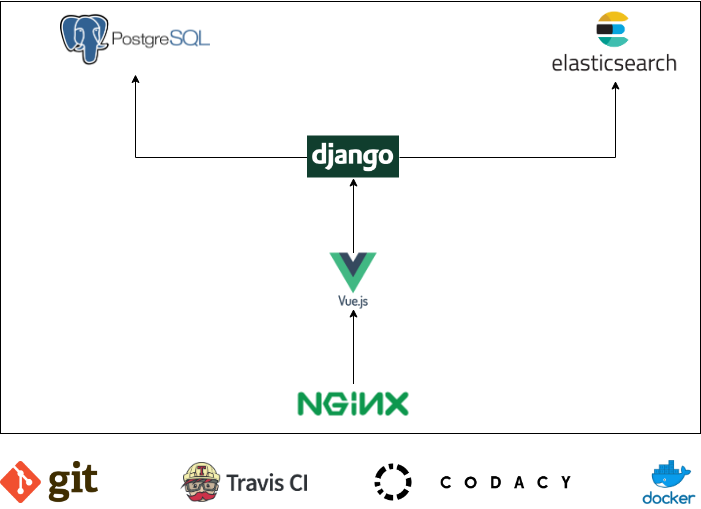
\includegraphics[height=\paperheight,width=\paperwidth]{img/architecture/architecture_diagram}}
			\setbeamertemplate{navigation symbols}{}
			\begin{frame}[plain]
			\end{frame}
		}
	
	\section{Implementación}
		\begin{frame}{Tecnologías}
			\begin{center}
				\smartdiagramset{circular distance=3cm, font=\large, text width=3.5cm, module minimum width=3.5cm, module minimum height=1.5cm, arrow tip=to}
				\smartdiagram[circular diagram]{Web Scrapping, Recuperación de información, Sistemas de recomendación}
			\end{center}
		\end{frame}

		\begin{frame}{Demo}
			\begin{center}
				
\includegraphics[width=\textwidth,height=0.5\textheight,keepaspectratio]{img/architecture/youtube}
			\end{center}
			\begin{center}
				\href{https://bit.ly/2ZqCkrJ}{\beamergotobutton{https://bit.ly/2ZqCkrJ}}
			\end{center}
		\end{frame}
\end{document}